\section{Modules}
\label{sec:Modules}
A Spring XD Module \cite{modules} is a unit of data processing. There are four module
types: source, processor, sink, and job. Modules in Spring XD are defined
in their own application context. This allows for easy encapsulation and life cycle
management for modules. Additionally, the use of an application context allows for easy
module expansion.  Spring XD uses Spring Integration \cite{spring-integration-reference}
as its foundation for implementing modules. A module is comprised of components that
implement the data processing logic and one or more connectors (known as channels)
that connect to the underlying message bus.

\par

Spring XD offers a suite of 23 sources, 24 sinks, 9 processors and 9 jobs that are ready
to use at startup.  These modules integrate with a variety of well known and popular
data stores and processing systems such as JDBC\cite{jdbc}, HDFS, MongoDB\cite{mongodb},
Spark, Kafka, RabbitMQ, Sqoop, etc.  If an existing module does not meet the needs of a
given use case, Spring XD supports custom modules.

Spring XD sink and source modules are Message Endpoints
\cite{enterprise-integration-pattern-message-endpoint}
that are responsible for sending data to and receiving data from external applications
respectively. A source is the entry point for data into the stream. A sink is
the module that dispatches the stream's results to an external application or storage system.
A processor module is used to modify data transmitted from the source to sink.
Multiple processors may be chained together. Batch jobs are used to execute batch
processing steps on a set of data.

\par

\subsection{Source}
\label{sec:Source}
Source modules receive inbound data and send to downstream modules in the stream or to a batch job
which could be triggered with the data. There are two source types: poller and event driven.
A poller source is based on the polling consumer pattern \cite{enterprise-integration-pattern-pollingconsumer}.
It polls an external application (such as a web service, FTP server, database) for data at a
configurable interval. An event driven source is based on the event driven
consumer pattern \cite{enterprise-integration-pattern-eventdrivenconsumer} which
opens a port to listen for incoming data that is pushed from an external application.

\par

In the case of a source module there is an ``output'' connector channel to dispatch data
transmitted by the module to a downstream module(see figure~\ref{fig:sourcembc}.)

\par

\begin{figure}[ht]
\centering
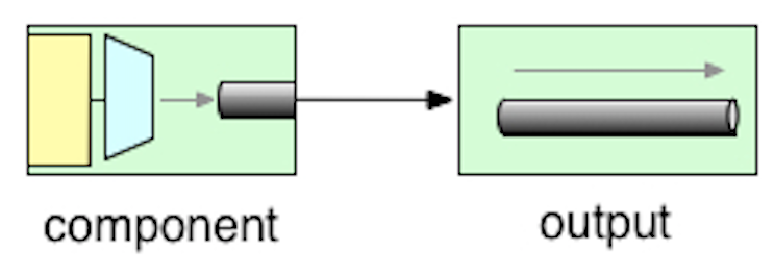
\epsfig{file=integration-module-output-channel.eps, height=.6in, width=1.75in}
\caption{Source Module Basic Components}
\label{fig:sourcembc}
\end{figure}

\par

\subsection{Processor}
\label{sec:Processor}
A processor is the module that receives data from a source or a previous processor
module's output, performs the transformation operation and sends the data
into a sink module or a downstream processor module. The basic processor
includes both ``input'' and ``output'' connector channels and the data processing component.
The input channel receives data from the upstream module and dispatches it to
the data processing component (see figure~\ref{fig:processormbc}.) It is the responsibility of
this component to transform the data. The transformed data is then sent to the downstream module
via the output channel.

\par

\begin{figure}
\centering
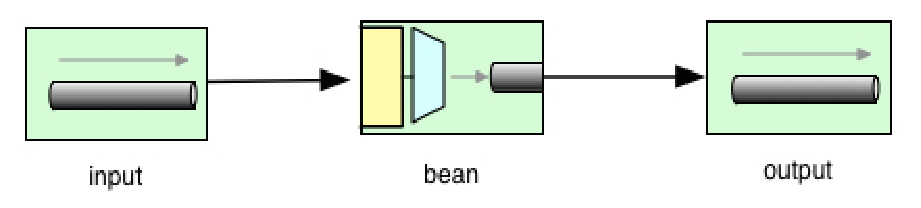
\epsfig{file=module-processor.eps, height=.6in, width=2.5in}
\caption{Processor Module Basic Components}
\label{fig:processormbc}
\end{figure}

\par

\subsection{Sink}
Sink modules convert and deliver data out of the stream in a format consumable by
an external application.  There are two types of sinks: analytic and delegate.
An analytic sink is used to perform analytic operations (such as count, gauge) on the
incoming data and store the result into a metric repository. (See section~\ref{sec:Analytics}.)
A delegate sink translates data to the format expected by the external application.
After transforming the data, the resulting data is sent to the external application.

\par

The basic sink includes an ``input'' channel connector and a data processing
component. The input channel receives data from the stream and dispatches
it to the data processing component which is responsible for connecting to the external
application(see figure~\ref{fig:sinkmbc}.) The sinks included with Spring XD have
configurable options for retries in case of failure.

\par

\begin{figure}
\centering

\epsfig{file=integration-module-input-channel.eps, height=.6in, width=1.75in}
\caption{Sink Module Basic Components}
\label{fig:sinkmbc}
\end{figure}

\par

\subsection{Job}
\label{sec:Job}
Spring XD uses Spring Batch \cite{spring-batch-reference}, a JSR standard (JSR-352)
for batch workload data processing as the foundation for implementing
job modules. A job enables users to execute enterprise batch processes within Spring XD.
Jobs are typically used when running long lasting tasks that have transactional requirements.
To account for failure scenarios, the workflow in the job can be designed to restart and
resume operation or roll-back the transaction altogether. A job can be triggered by the
stream with the data that act as the input to start the batch processing. This makes
streams and job modules unified under a single platform.

\par

A job typically consists of a job definition along with the supporting
data processing components as shown in figure~\ref{fig:batchmbc}.
In some cases the job definition alone is sufficient to implement the desired behavior.

\par

\begin{figure}
\centering
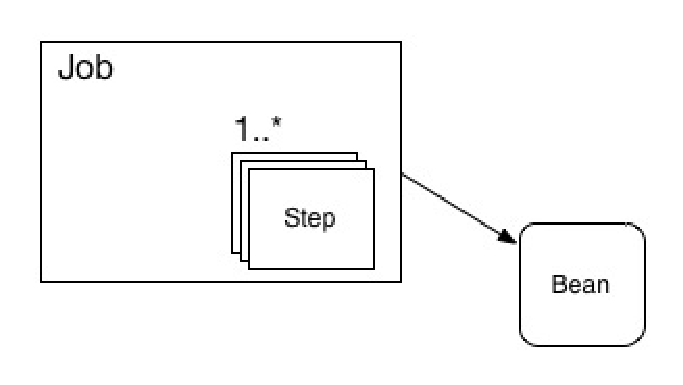
\epsfig{file=integration-batch.eps, height=.8in, width=2in}
\caption{Batch Basic Components}
\label{fig:batchmbc}
\end{figure}

\par 

\subsection{Composite}
A composite module provides a way to create a single module that contains
multiple modules. A composite module can be used to prevent
duplication when a processing chain of modules is used frequently.
Additionally, data passed between modules in a composite module will be
transmitted in memory (as opposed to the message bus) -- thus improving
performance.

\par

\subsection{Module Registry}
The module registry is where Spring XD looks for modules during
deployment. A module can be bundled as an archive or defined along with its
dependencies inside the module registry. The modules are defined in
the modules directory and are segregated in subdirectories by
type: \texttt{modules/source}, \texttt{modules/processor},
\texttt{modules/sink} and \texttt{modules/job}. The module registry is
configurable and modules may be uploaded via the admin server REST API.
During the deployment of the module, the Spring XD runtime will load the modules
dynamically from the module registry.
